% ==========================================
% BAB IV PERANCANGAN
% ==========================================
\cleardoublepage
\chapter{PERANCANGAN}
\label{chap:perancangan}

\section{Diagram Arsitektur}
Subbab ini menjabarkan arsitektur sistem \textit{Smart Warehouse} secara bertingkat, dari gambaran sistem keseluruhan pada Level 0 hingga dekomposisi komponen perangkat lunak yang menyusun \textit{Warehouse Management Controller} (WMC) pada Level 2. Fokus pembahasan diarahkan pada WMC sebagai subsistem perangkat lunak yang dikembangkan, beserta komponen-komponen yang secara langsung berinteraksi dengannya.

\subsection{Arsitektur Level 0}
Arsitektur Level 0 menggambarkan sistem \textit{Smart Warehouse} secara menyeluruh sebagai satu kesatuan modul tunggal. Pada level ini, sistem dipandang sebagai kotak hitam (\textit{black box}) yang menerima berbagai masukan dari lingkungan eksternal dan menghasilkan keluaran berupa eksekusi fisik pemindahan barang serta laporan status operasional. Sistem ini berinteraksi langsung dengan staf gudang (\textit{Warehouse Staff}) dan sistem logistik eksternal. Tabel \ref{tab:level0} merangkum fungsi, masukan, dan keluaran sistem pada arsitektur Level 0.

\begin{table}[h]
  \centering
  \caption{Fungsi, masukan, dan keluaran sistem \textit{Smart Warehouse} (Level 0)}
  \label{tab:level0}
  \begin{tabularx}{\textwidth}{ | l | X | }
    \hline
    \textbf{Elemen} & \textbf{Deskripsi} \\
    \hline
    Modul & Sistem \textit{Smart Warehouse} (\textit{Finished Goods}) \\
    \hline
    Fungsi & Melakukan interaksi perintah \textit{picking} dan \textit{storing} serta data yang dikirimkan dari \textit{Warehouse Staff}, serta melakukan integrasi data gudang dengan sistem yang sudah ada. \\
    \hline
    Masukan & 1. \textit{Warehouse data} --- informasi stok, lokasi penyimpanan, dan status barang dari sistem eksternal. 2. \textit{Requested item} --- permintaan pengambilan barang dari \textit{Warehouse Staff}. 3. \textit{Item for storing} --- barang fisik yang akan disimpan beserta data ID barang. 4. \textit{Warehouse condition report} --- kapasitas ruang, posisi rak, dan kondisi area penyimpanan. \\
    \hline
    Luaran & 1. \textit{Order status} --- informasi keberhasilan proses ke operator dan sistem. 2. \textit{Robots data} --- status operasi robot, progres navigasi, dan hasil tugas. 3. \textit{Goods delivery} --- barang fisik yang dikirim ke sistem logistik. 4. \textit{Logistic documentation} --- laporan pelepasan barang dan dokumen \textit{tracking}. \\
    \hline
  \end{tabularx}
\end{table}

\subsection{Arsitektur Level 1 --- Warehouse Management Controller}
Pada Level 1, sistem \textit{Smart Warehouse} didekomposisi menjadi dua subsistem utama, yaitu \textit{Goods Handling and Delivery System} (GHDS) yang menangani aktivitas fisik robot, dan \textit{Warehouse Management Controller} (WMC) yang menjadi fokus pengembangan pada tugas akhir ini. WMC berfungsi sebagai pusat kendali digital yang mengelola permintaan barang, mengoordinasikan pengendalian robot, serta memperbarui status pesanan secara terintegrasi. WMC berinteraksi langsung dengan antarmuka pengguna, basis data, dan \textit{Fleet Controller} pada GHDS. Tabel \ref{tab:level1} merangkum fungsi, masukan, dan keluaran WMC pada Level 1.

\begin{table}[h]
  \centering
  \caption{Fungsi, masukan, dan keluaran \textit{Warehouse Management Controller} (Level 1)}
  \label{tab:level1}
  \begin{tabularx}{\textwidth}{ | l | X | }
    \hline
    \textbf{Elemen} & \textbf{Deskripsi} \\
    \hline
    Fungsi & Mengelola dan mengkoordinasikan proses permintaan barang, pengendalian robot, serta pembaruan status pesanan di gudang secara terintegrasi. \\
    \hline
    Masukan & 1. Data robot --- informasi kondisi, posisi, dan status operasional robot. 2. Status pesanan --- informasi perkembangan pesanan yang sedang diproses. 3. Permintaan barang --- permintaan pengambilan atau penyediaan barang dari gudang. 4. Perintah pesanan --- instruksi untuk memproses atau mengeksekusi pesanan tertentu. 5. Kredensial --- data autentikasi untuk memverifikasi akses pengguna. \\
    \hline
    Luaran & 1. Barang yang diminta --- informasi atau perintah terkait barang yang harus diambil atau disiapkan. 2. Informasi \& data robot --- kondisi dan data operasional robot yang telah diperbarui. 3. Status pesanan --- status terbaru pesanan setelah diproses oleh sistem. 4. \textit{Bearer Token} --- token autentikasi untuk mengamankan komunikasi antar layanan. \\
    \hline
  \end{tabularx}
\end{table}

\subsection{Arsitektur Level 2 --- Komponen Warehouse Management Controller}
Pada Level 2, WMC didekomposisi menjadi empat komponen perangkat lunak yang masing-masing memiliki tanggung jawab yang terdefinisi. Keempat komponen tersebut adalah \textit{Database}, \textit{Goods Detail Service}, \textit{Fleet Order Service}, dan \textit{Authentication Service}. Setiap komponen saling terhubung dan beroperasi dalam arsitektur \textit{microservices} yang memungkinkan setiap layanan dikembangkan dan di-\textit{deploy} secara independen (lihat Subbab \ref{chap:studi-literatur} tentang arsitektur \textit{microservices}, khususnya Gambar \ref{fig:microservices-diagram}).

\subsubsection{Database}
Komponen \textit{Database} merupakan lapisan penyimpanan data terpusat pada WMC. Komponen ini menyimpan seluruh data operasional gudang, mencakup detail barang, \textit{layout} penyimpanan, data pengguna, sesi autentikasi, dan status pengiriman robot. Seluruh layanan WMC lainnya berinteraksi dengan komponen ini melalui mekanisme \textit{query} yang terstruktur. Tabel \ref{tab:database-io} merangkum fungsi, masukan, dan keluaran komponen \textit{Database}.

\begin{table}[h]
  \centering
  \caption{Fungsi, masukan, dan keluaran \textit{Database} WMC}
  \label{tab:database-io}
  \begin{tabularx}{\textwidth}{ | l | X | }
    \hline
    \textbf{Elemen} & \textbf{Deskripsi} \\
    \hline
    Fungsi & Menyimpan dan menyediakan data keseluruhan operasional gudang, mencakup detail barang, \textit{layout} penyimpanan, status pengiriman robot, data pengguna, dan sesi autentikasi. \\
    \hline
    Masukan & 1. \textit{Query Data Goods} --- permintaan baca/ubah/hapus data barang dari \textit{Goods Detail Service}. 2. \textit{Auth Query} / \textit{Session Data} --- diterima dari \textit{Authentication Service} untuk validasi pengguna dan penyimpanan sesi. 3. \textit{Location Query} \& \textit{Order Data} --- diterima dari \textit{Fleet Order Service} untuk mendapatkan lokasi barang dan memperbarui detail barang. \\
    \hline
    Luaran & 1. \textit{Goods Data} --- dikirim ke \textit{Goods Detail Service} sebagai hasil \textit{query} data barang. 2. \textit{User Data} / \textit{Session Info} --- dikirim ke \textit{Authentication Service}. 3. \textit{Location Data} / \textit{Updated Goods Detail} --- dikirim ke \textit{Fleet Order Service}. \\
    \hline
  \end{tabularx}
\end{table}

\subsubsection{Goods Detail Service}
Komponen \textit{Goods Detail Service} bertanggung jawab mengelola data master seluruh barang yang tersimpan di gudang. Komponen ini menjadi antarmuka antara \textit{Database} dan komponen lain yang memerlukan informasi barang, mencakup penyimpanan, pembaruan, dan pengambilan informasi secara terperinci. Tabel \ref{tab:gds-io} merangkum fungsi, masukan, dan keluaran komponen ini.

\begin{table}[h]
  \centering
  \caption{Fungsi, masukan, dan keluaran \textit{Goods Detail Service} WMC}
  \label{tab:gds-io}
  \begin{tabularx}{\textwidth}{ | l | X | }
    \hline
    \textbf{Elemen} & \textbf{Deskripsi} \\
    \hline
    Fungsi & Mengelola data master seluruh barang di gudang, mencakup penyimpanan, pembaruan, dan pengambilan informasi barang secara terperinci. \\
    \hline
    Masukan & 1. \textit{Goods Data} --- objek data berisi informasi lengkap atau pembaruan detail satu atau lebih item barang. 2. \textit{Query Data} --- permintaan spesifik untuk mengambil, menghapus, atau memverifikasi detail barang. \\
    \hline
    Luaran & 1. \textit{Goods Data} --- data barang sebagai respons atas permintaan \textit{Query Data}. 2. \textit{Query Data} --- respons konfirmasi bahwa permintaan telah dieksekusi. \\
    \hline
  \end{tabularx}
\end{table}

\subsubsection{Fleet Order Service}
Komponen \textit{Fleet Order Service} merupakan \textit{gateway} utama antara sistem WMC dan komponen \textit{Fleet Controller} pada robot. Komponen ini mengolah seluruh logika pembuatan dan pembatalan \textit{order}, pengaturan tugas robot, serta pemantauan dan sinkronisasi status tugas secara \textit{real-time}. Tabel \ref{tab:fos-io} merangkum fungsi, masukan, dan keluaran komponen ini.

\begin{table}[h]
  \centering
  \caption{Fungsi, masukan, dan keluaran \textit{Fleet Order Service} WMC}
  \label{tab:fos-io}
  \begin{tabularx}{\textwidth}{ | l | X | }
    \hline
    \textbf{Elemen} & \textbf{Deskripsi} \\
    \hline
    Fungsi & Mengolah seluruh data dan logika pembuatan \textit{order}, pengaturan tugas robot, pemantauan status robot, serta sinkronisasi status tugas. Menjadi \textit{gateway} antara sistem internal WMC dan \textit{Fleet Controller}. \\
    \hline
    Masukan & 1. \textit{Order Command} --- instruksi pembuatan atau pembatalan \textit{order} dari antarmuka pengguna. 2. \textit{Robot Status} \& \textit{Task Status} --- informasi posisi, baterai, \textit{error}, dan progres tugas dari \textit{Fleet Controller}. 3. \textit{Order Data} / \textit{Location Data} --- diterima dari \textit{Database} untuk memproses dan memperbarui catatan \textit{order}. \\
    \hline
    Luaran & 1. \textit{Order Status Event} --- dikirim ke antarmuka pengguna sebagai respons status \textit{order} terkini. 2. \textit{Command} ke \textit{Fleet Controller} --- instruksi robot berupa \textit{start task}, \textit{cancel task}, atau \textit{emergency stop}. 3. \textit{Updated Goods Detail} --- dikirim ke \textit{Database} setelah \textit{order} diproses. \\
    \hline
  \end{tabularx}
\end{table}

\subsubsection{Authentication Service}
Komponen \textit{Authentication Service} bertanggung jawab memvalidasi identitas pengguna yang mengakses sistem WMC. Komponen ini menerima kredensial dari antarmuka pengguna, memverifikasinya terhadap data pada \textit{Database}, kemudian menerbitkan \textit{Bearer Token} sebagai bukti otorisasi untuk seluruh permintaan berikutnya. Tabel \ref{tab:auth-io} merangkum fungsi, masukan, dan keluaran komponen ini.

\begin{table}[h]
  \centering
  \caption{Fungsi, masukan, dan keluaran \textit{Authentication Service} WMC}
  \label{tab:auth-io}
  \begin{tabularx}{\textwidth}{ | l | X | }
    \hline
    \textbf{Elemen} & \textbf{Deskripsi} \\
    \hline
    Fungsi & Memvalidasi identitas pengguna berdasarkan kredensial yang diberikan, menghasilkan token autentikasi (\textit{Bearer Token}), serta mengelola sesi pengguna. \\
    \hline
    Masukan & 1. \textit{Credential} Pengguna --- data \textit{username} dan \textit{password} diterima dari antarmuka pengguna via API HTTP/HTTPS. 2. \textit{Session Info} / \textit{User Data} --- hasil pencarian pengguna dari \textit{Database}. 3. \textit{Token} / \textit{Session ID} (opsional) --- diterima dari antarmuka pengguna untuk validasi sesi yang masih aktif. \\
    \hline
    Luaran & 1. \textit{Bearer Token} --- dikirim ke antarmuka pengguna sebagai \textit{string} token untuk otorisasi permintaan berikutnya. 2. \textit{Session Data} --- dikirim ke \textit{Database} untuk disimpan atau diperbarui. 3. Informasi Penolakan Akses --- pesan kesalahan dikirim ke antarmuka pengguna bila kredensial tidak valid atau sesi telah kedaluwarsa. \\
    \hline
  \end{tabularx}
\end{table}

\subsection{Desain Subsistem Lokalisasi}
Subsistem Lokalisasi merupakan komponen perangkat lunak yang berada di dalam \textit{Fleet Controller}, berjalan secara paralel dengan \textit{Navigation subsystem} pada robot. Jika \textit{Navigation subsystem} menentukan posisi robot dari perspektif internal robot melalui pembacaan kode QR di lantai dan sensor IMU, Subsistem Lokalisasi menyediakan perspektif eksternal dari atas (\textit{overhead}) yang mencakup seluruh area lantai gudang sekaligus---termasuk posisi robot, barang, dan \textit{docking station}. \textit{Output} subsistem ini berupa data \textit{grid state} yang dipublikasikan melalui MQTT ke \textit{topic location} pada RabbitMQ \textit{broker}, dikonsumsi oleh \textit{Fleet Manager} untuk keperluan \textit{digital twin} koordinasi robot, serta oleh \textit{Fleet Order Service} di WMC untuk diteruskan ke \textit{User Interface} secara \textit{real-time}.

\subsubsection{Perangkat Lokalisasi}
Perangkat lokalisasi adalah rakitan kamera \textit{overhead} yang dipasang setinggi 60 cm di atas lantai gudang berukuran $2,4 \times 1,2$ m. Rakitan ini terdiri dari rangka penyangga, sebuah kamera IP \textit{fisheye} berkemampuan 1080p (3 MP) dengan \textit{H.264 encoding} yang melakukan \textit{streaming} melalui protokol RTSP \textit{over} TCP, serta pencahayaan LED tambahan untuk memastikan iluminasi yang seragam di seluruh area lantai. Optik \textit{fisheye} dipilih karena kemampuannya mencakup seluruh area lantai gudang dari satu titik pemasangan tunggal tanpa oklusi, meskipun memerlukan proses koreksi distorsi sebelum dapat digunakan untuk pemetaan posisi yang akurat (lihat Subbab 2.5.2).

\subsubsection{Desain Pipeline Deteksi}
Subsistem Lokalisasi didesain sebagai \textit{pipeline} pemrosesan \textit{frame} yang berjalan secara kontinu. Sebuah \textit{background thread} mengambil \textit{frame} terbaru dari \textit{stream} RTSP secara terus-menerus dan membuang \textit{frame} yang sudah basi, sementara \textit{detection loop} utama berjalan pada frekuensi 4 Hz. Setiap \textit{frame} diproses melalui enam tahap secara berurutan, sebagaimana dirangkum pada Tabel \ref{tab:pipeline-lokalisasi}.

\begin{table}[h]
  \centering
  \caption{\textit{Pipeline} pemrosesan Subsistem Lokalisasi}
  \label{tab:pipeline-lokalisasi}
  \begin{tabularx}{\textwidth}{ | c | l | X | }
    \hline
    \textbf{No.} & \textbf{Tahap} & \textbf{Deskripsi} \\
    \hline
    1 & Koreksi Distorsi Lensa & Menghilangkan distorsi radial \textit{fisheye} menggunakan koefisien kalibrasi Kannala--Brandt yang dihitung saat \textit{setup}. \\
    \hline
    2 & Pra-pemrosesan & Meningkatkan kontras \textit{frame} yang telah terkoreksi dan mengonversinya ke \textit{grayscale} untuk detektor. \\
    \hline
    3 & Deteksi AprilTag & Menjalankan detektor Tag36h11 (\textit{marker} fisik $8\times8$ cm) untuk mengekstrak ID, posisi piksel pusat, dan empat koordinat sudut setiap \textit{tag}. \\
    \hline
    4 & Pemetaan Grid & Mentransformasi koordinat piksel ke sel \textit{grid} diskrit menggunakan \textit{homography} $H$ dan aturan \textit{nearest-cell-centre} (lihat Subbab 2.5.3). \\
    \hline
    5 & Klasifikasi dan Heading & Mengklasifikasikan setiap \textit{tag} ID ke salah satu dari tiga kategori: \textit{docking station}, robot, atau \textit{warehouse item}. Orientasi (\textit{heading} $0^\circ$--$359^\circ$) diperoleh dari sudut sisi depan \textit{tag}. \\
    \hline
    6 & Publikasi MQTT & Mengodekan seluruh \textit{grid occupancy state} sebagai \textit{payload} JSON dan mempublikasikannya setiap 500 ms ke \textit{topic location} pada RabbitMQ \textit{broker}. \\
    \hline
  \end{tabularx}
\end{table}

\subsection{Desain Real-Time Streaming via WebSocket}
Untuk menyampaikan telemetri \textit{order} dan robot secara langsung ke \textit{User Interface} tanpa mekanisme \textit{polling}, \textit{Fleet Order Service} mengekspos sebuah WebSocket server yang memungkinkan koneksi persisten dua arah antara server dan klien UI. Pendekatan ini dipilih untuk memenuhi KNF-02 yang menetapkan pembaruan status robot harus tersedia di UI dalam kurun waktu $\leq$1 detik dari kejadian sesungguhnya, sebuah target yang tidak dapat dicapai secara andal melalui REST \textit{polling} periodik.

Pada saat koneksi WebSocket terbentuk, UI berlangganan pada dua \textit{data stream} secara bersamaan. Pertama, \textit{order stream} mendorong transisi status \textit{order} secara \textit{real-time} (\texttt{PENDING} $\rightarrow$ \texttt{IN\_PROGRESS} $\rightarrow$ \texttt{COMPLETED}) setiap kali \textit{Fleet Order Service} memproses perubahan \textit{state order}. Kedua, \textit{robot stream} meneruskan koordinat \textit{grid} dan orientasi robot terbaru yang diterima dari \textit{topic} MQTT \textit{location}, melakukan \textit{broadcast payload} terbaru ke seluruh klien yang terhubung dalam satu siklus \textit{publish} MQTT. Dengan demikian, latensi tampilan posisi robot di UI terikat langsung pada interval publikasi Subsistem Lokalisasi (500 ms), jauh di bawah target KNF-02 sebesar 1 detik.

\section{Desain Basis Data}
\textit{Entity Relationship Diagram} (ERD) adalah diagram yang menggambarkan struktur data dalam suatu sistem informasi yang berguna untuk mengetahui hubungan antar entitas, atribut dari masing-masing entitas, dan apa saja entitas yang berperan di dalam penyimpanan data \autocite{silberschatz2020}. ERD merupakan bagian penting dalam proses perancangan sistem, khususnya dalam merancang skema basis data relasional yang terstruktur dan konsisten.

Pada tugas akhir ini, ERD digunakan untuk memodelkan entitas-entitas utama yang terlibat dalam sistem \textit{Warehouse Management Controller}, yaitu \textit{User}, \textit{Session}, \textit{Order}, \textit{OrderItem}, \textit{Item}, \textit{ItemLocation}, \textit{Task}, \textit{Robot}, dan \textit{RobotLog}, beserta seluruh relasi yang menghubungkan entitas-entitas tersebut. Entitas-entitas ini saling terhubung secara relasional sesuai dengan pendekatan basis data SQL yang diterapkan pada sistem. Berdasarkan pemodelan tersebut, terdapat sembilan entitas yang dirancang dalam basis data sistem. Entitas \textit{User} menyimpan data pengguna sistem beserta kredensial autentikasi, sedangkan entitas \textit{Session} mencatat informasi sesi aktif pengguna termasuk token dan masa berlakunya. Entitas \textit{Order} merepresentasikan setiap permintaan \textit{picking} maupun \textit{storing} yang dibuat oleh pengguna, dan terhubung dengan entitas \textit{OrderItem} yang memuat rincian barang dalam setiap \textit{order} beserta kuantitasnya. Entitas \textit{Item} menjadi master data barang yang tersimpan di gudang, dilengkapi dengan entitas \textit{ItemLocation} untuk menyimpan informasi posisi fisik barang berupa koordinat rak dalam area gudang. Entitas \textit{Task} menghubungkan \textit{OrderItem} dengan \textit{Robot}, merepresentasikan instruksi operasional yang diberikan kepada robot untuk dieksekusi. Entitas \textit{Robot} menyimpan data identitas dan kapasitas robot, sementara entitas \textit{RobotLog} mencatat seluruh aktivitas dan kejadian pada setiap robot sebagai mekanisme \textit{logging} dan pelacakan kesalahan sistem.

\subsection{Entitas User}
Entitas \textit{User} berguna untuk menyimpan data pengguna sistem yang merupakan staf gudang yang bertugas mengelola dan memantau seluruh operasional \textit{Warehouse Management Controller}. Struktur data dari entitas \textit{User} mencakup informasi identitas pengguna seperti nama, \textit{username}, dan \textit{password} yang digunakan untuk keperluan autentikasi, serta \textit{timestamp} pembuatan, pembaruan, dan penghapusan data. Entitas \textit{User} terhubung dengan dua entitas lain dalam sistem. Relasi dengan entitas \textit{Order} memungkinkan sistem melacak seluruh permintaan \textit{picking} dan \textit{storing} yang dibuat oleh masing-masing pengguna, sedangkan relasi dengan entitas \textit{Session} digunakan untuk mengelola sesi login aktif pengguna berdasarkan token autentikasi yang diterbitkan setelah proses login berhasil dilakukan.

\subsection{Entitas Order}
Entitas \textit{Order} berguna untuk menyimpan data permintaan operasional gudang yang diajukan oleh pengguna, baik berupa proses \textit{picking} (pengambilan barang) maupun \textit{storing} (penyimpanan barang). Struktur data dari entitas \textit{Order} mencakup referensi pengguna yang mengajukan permintaan, status terkini dari permintaan tersebut, serta \textit{timestamp} pembuatan, pembaruan, dan penghapusan data. Entitas \textit{Order} terhubung dengan dua entitas lain dalam sistem. Relasi dengan entitas \textit{User} mengikat setiap permintaan kepada pengguna yang membuatnya sehingga sistem dapat melakukan pelacakan dan audit aktivitas secara terstruktur, sedangkan relasi dengan entitas \textit{OrderItem} memungkinkan satu permintaan mencakup beberapa barang sekaligus dengan rincian kuantitas masing-masing.

Status \textit{Order} berubah mengikuti alur \textit{state machine} yang dipublikasikan secara \textit{real-time} ke \textit{User Interface} melalui WebSocket, sebagaimana diilustrasikan pada Gambar \ref{fig:order-statechart}.

\begin{figure}[h]
  \caption{\textit{Statechart} transisi status entitas \textit{Order}}
  \label{fig:order-statechart}
  \centering
  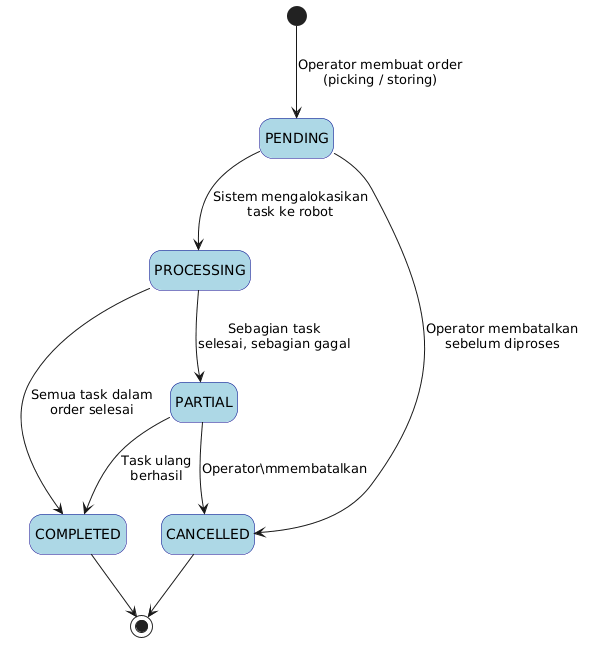
\includegraphics[width=0.6\textwidth]{images/order_sc.png}
\end{figure}

\subsection{Entitas OrderItem}
Entitas \textit{OrderItem} berguna untuk menyimpan data rincian barang yang terdapat dalam suatu permintaan operasional gudang. Struktur data dari entitas \textit{OrderItem} mencakup referensi ke permintaan induk, referensi ke barang yang diminta, jumlah kuantitas yang diperlukan, serta \textit{timestamp} pembuatan, pembaruan, dan penghapusan data. Entitas \textit{OrderItem} merupakan entitas penghubung yang memiliki relasi dengan tiga entitas sekaligus dalam sistem. Relasi dengan entitas \textit{Order} mengaitkan setiap detail barang ke permintaan asalnya, relasi dengan entitas \textit{Item} menentukan barang spesifik yang menjadi objek permintaan, sedangkan relasi dengan entitas \textit{Task} menjadi dasar pembentukan instruksi operasional yang akan diberikan kepada robot untuk dieksekusi.

\subsection{Entitas Item}
Entitas \textit{Item} berguna untuk menyimpan master data seluruh barang yang dikelola di dalam gudang. Struktur data dari entitas \textit{Item} mencakup informasi identitas barang seperti nama, deskripsi, \textit{stock-keeping unit} (SKU), kategori, dan jumlah stok yang tersedia, serta \textit{timestamp} pembuatan, pembaruan, dan penghapusan data. Entitas \textit{Item} terhubung dengan dua entitas lain dalam sistem. Relasi dengan entitas \textit{OrderItem} memungkinkan sistem merujuk data barang secara akurat ketika memproses permintaan operasional, sedangkan relasi dengan entitas \textit{ItemLocation} digunakan untuk menyimpan informasi posisi fisik barang di dalam gudang berupa koordinat rak sehingga robot dapat menavigasi ke lokasi yang tepat.

\subsection{Entitas Task}
Entitas \textit{Task} berguna untuk menyimpan data instruksi operasional yang diberikan kepada robot sebagai tindak lanjut dari permintaan \textit{picking} atau \textit{storing} yang masuk ke sistem. Struktur data dari entitas \textit{Task} mencakup referensi ke detail permintaan barang yang harus dikerjakan, referensi ke robot yang ditugaskan, status pelaksanaan tugas, serta \textit{timestamp} pembuatan, pembaruan, dan penghapusan data. Entitas \textit{Task} terhubung dengan dua entitas lain dalam sistem. Relasi dengan entitas \textit{OrderItem} mengaitkan setiap instruksi dengan permintaan barang yang harus diselesaikan, sedangkan relasi dengan entitas \textit{Robot} menentukan robot mana yang bertanggung jawab mengeksekusi tugas tersebut sehingga sistem dapat melakukan pemantauan dan pengelolaan armada robot secara terpusat.

Status \textit{Task} mengikuti alur \textit{state machine} sebagaimana diilustrasikan pada Gambar \ref{fig:task-statechart}.

\begin{figure}[h]
  \caption{\textit{Statechart} transisi status entitas \textit{Task}}
  \label{fig:task-statechart}
  \centering
  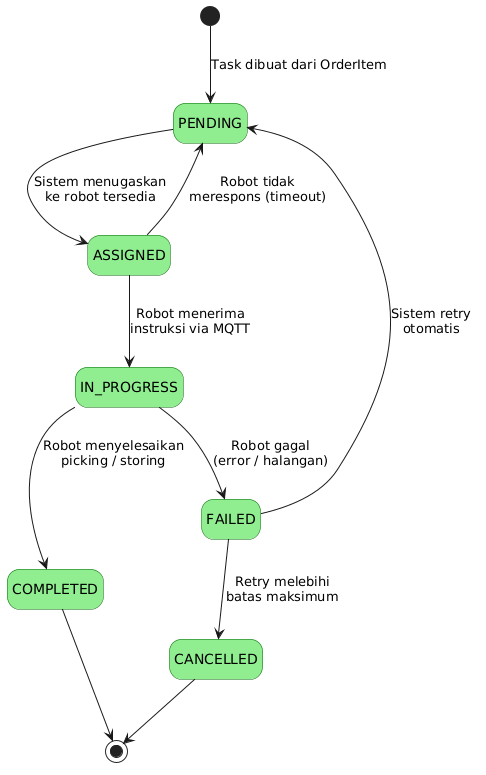
\includegraphics[width=0.6\textwidth]{images/task_sc.png}
\end{figure}

\subsection{Entitas Robot}
Entitas \textit{Robot} berguna untuk menyimpan data identitas dan kapasitas setiap unit robot yang beroperasi di dalam gudang. Struktur data dari entitas \textit{Robot} mencakup nomor seri robot, kapasitas muatan maksimum, kapasitas baterai, serta waktu pemeliharaan terakhir yang dilakukan. Entitas \textit{Robot} terhubung dengan dua entitas lain dalam sistem. Relasi dengan entitas \textit{Task} memungkinkan sistem menugaskan dan memantau seluruh instruksi operasional yang sedang dijalankan oleh masing-masing robot, sedangkan relasi dengan entitas \textit{RobotLog} digunakan untuk mencatat seluruh aktivitas, kode log, kode kesalahan, dan pesan kejadian yang terjadi pada robot selama beroperasi sebagai mekanisme \textit{logging} dan penelusuran kesalahan sistem.

Status operasional \textit{Robot} (\textit{idle}/\textit{active}/\textit{charging}/\textit{error}) mengikuti alur \textit{state machine} sebagaimana diilustrasikan pada Gambar \ref{fig:robot-statechart}.

\begin{figure}[h]
  \caption{\textit{Statechart} transisi status entitas \textit{Robot}}
  \label{fig:robot-statechart}
  \centering
  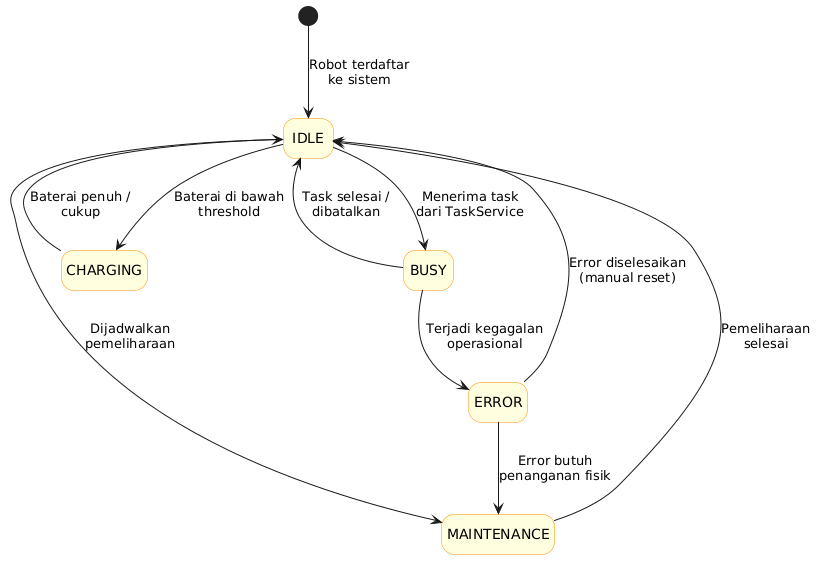
\includegraphics[width=0.6\textwidth]{images/robot_sc.png}
\end{figure}

\subsection{Entitas Session}
Entitas \textit{Session} berguna untuk menyimpan informasi sesi aktif setiap pengguna yang berhasil melakukan autentikasi ke dalam sistem. Struktur data entitas \textit{Session} mencakup token sesi, waktu kedaluwarsa (\textit{expiry}), serta status validitas token yang digunakan untuk memverifikasi kredensial pengguna pada setiap permintaan yang dikirimkan ke layanan WMC. Entitas \textit{Session} terhubung dengan entitas \textit{User} melalui relasi \textit{one-to-many}, di mana satu pengguna dapat memiliki beberapa sesi aktif secara bersamaan, namun setiap sesi selalu dimiliki oleh tepat satu pengguna.

\subsection{Entitas ItemLocation}
Entitas \textit{ItemLocation} berguna untuk menyimpan informasi posisi fisik setiap jenis barang dalam area gudang, direpresentasikan sebagai koordinat sel pada \textit{grid} lantai gudang. Struktur data entitas \textit{ItemLocation} mencakup koordinat kolom ($c$) dan baris ($r$) pada \textit{grid} $8\times4$ yang merepresentasikan posisi penyimpanan barang, serta stempel waktu pembaruan terakhir untuk keperluan \textit{traceability} lokasi. Entitas ini terhubung dengan entitas \textit{Item} melalui relasi \textit{one-to-one}, memastikan bahwa setiap jenis barang selalu memiliki satu catatan lokasi aktif yang dapat diperbarui secara \textit{real-time} mengikuti perpindahan barang oleh robot.

\subsection{Entitas RobotLog}
Entitas \textit{RobotLog} berguna untuk mencatat seluruh kejadian, aktivitas, dan kesalahan yang terjadi pada setiap robot selama beroperasi di dalam gudang sebagai mekanisme \textit{logging} dan \textit{audit trail}. Struktur data entitas \textit{RobotLog} mencakup kode log, kode kesalahan (\textit{error code}), pesan kejadian, serta stempel waktu kejadian. Entitas \textit{RobotLog} terhubung dengan dua entitas lain: relasi dengan entitas \textit{Robot} (\textit{many-to-one}) untuk mengidentifikasi unit robot yang menghasilkan log, serta relasi dengan entitas \textit{Task} (\textit{many-to-one}) untuk mengaitkan setiap entri log dengan \textit{task} operasional yang sedang dijalankan saat kejadian tersebut terjadi, sehingga memudahkan penelusuran akar masalah (\textit{root cause analysis}) ketika terjadi kegagalan operasional.

\section{Kebutuhan Fungsional Sistem}
Kebutuhan fungsional sistem mendefinisikan kapabilitas spesifik yang harus tersedia bagi pengguna dalam berinteraksi dengan sistem \textit{Warehouse Management Controller}. Kebutuhan ini diturunkan langsung dari Tabel \ref{tab:kebutuhan-fungsional} dengan perincian yang lebih granular, sehingga setiap kebutuhan merepresentasikan satu fungsi yang dapat diuji secara mandiri. Tabel \ref{tab:kf-detail} merangkum kebutuhan fungsional yang diidentifikasi untuk mendukung pengembangan sistem \textit{Warehouse Management Controller} sebagai perangkat lunak pengelola operasional gudang berbasis robot.

\begin{table}[h]
  \centering
  \caption{Kebutuhan fungsional sistem \textit{Warehouse Management Controller}}
  \label{tab:kf-detail}
  \begin{tabularx}{\textwidth}{ | l | X | }
    \hline
    \textbf{Kode KF} & \textbf{Deskripsi Kebutuhan Fungsional} \\
    \hline
    KF-01 & Pengguna dapat melakukan login menggunakan \textit{username} dan \textit{password} yang terdaftar untuk mengakses sistem WMC. \\
    \hline
    KF-02 & Pengguna dapat melakukan \textit{logout} untuk mengakhiri sesi aktif dan keluar dari sistem secara aman. \\
    \hline
    KF-03 & Pengguna dapat melihat daftar seluruh barang di gudang beserta informasi ringkas: nama, SKU, kategori, dan stok. \\
    \hline
    KF-04 & Pengguna dapat melihat informasi lengkap suatu barang, termasuk atribut, dimensi, berat, dan kondisi stok. \\
    \hline
    KF-05 & Pengguna dapat melihat lokasi penyimpanan fisik barang di gudang: zona, rak, dan slot penyimpanan. \\
    \hline
    KF-06 & Pengguna dapat membuat \textit{order picking} untuk meminta robot mengambil barang dari lokasi penyimpanan ke titik keluaran gudang. \\
    \hline
    KF-07 & Pengguna dapat membuat \textit{order storing} untuk meminta robot menyimpan barang dari titik masuk ke lokasi penyimpanan yang sesuai. \\
    \hline
    KF-08 & Pengguna dapat melihat daftar seluruh \textit{order} beserta status perkembangannya secara \textit{real-time}. \\
    \hline
    KF-09 & Pengguna dapat memantau status seluruh \textit{task} robot yang aktif maupun selesai, termasuk log aktivitas eksekusi. \\
    \hline
    KF-10 & Pengguna dapat memantau kondisi operasional seluruh robot yang terdaftar dalam sistem, termasuk status dan histori aktivitas. \\
    \hline
  \end{tabularx}
\end{table}

\section{Skenario Use Case}
Skenario \textit{use case} mendeskripsikan interaksi antara pengguna dan sistem \textit{Warehouse Management Controller} (WMC) untuk setiap kebutuhan fungsional. Setiap skenario mencakup kondisi awal, kondisi akhir, langkah-langkah interaksi normal, serta skenario alternatif apabila terjadi kondisi di luar alur utama. Gambar \ref{fig:use-case-diagram} menyajikan diagram \textit{use case} yang merangkum seluruh interaksi aktor Pengguna (Operator Gudang) dengan sistem WMC.

\begin{figure}[t]
  \caption{Diagram \textit{use case} sistem \textit{Warehouse Management Controller}}
  \label{fig:use-case-diagram}
  \centering
  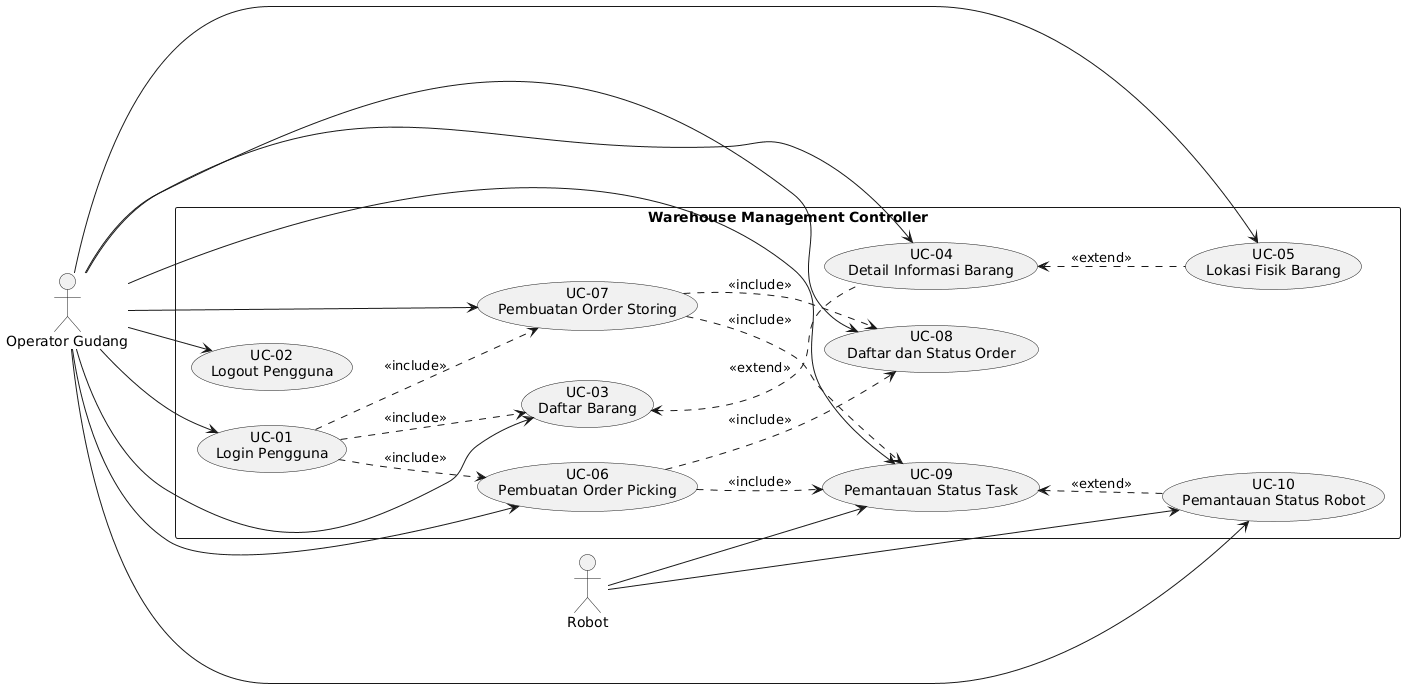
\includegraphics[width=0.9\textwidth]{images/use_case_diagram.png}
\end{figure}

\subsection{UC-01: Login Pengguna}
Tabel \ref{tab:uc01} menyajikan skenario UC-01: Login Pengguna.

\begin{table}[h]
  \centering
  \caption{Skenario UC-01: Login Pengguna}
  \label{tab:uc01}
  \begin{tabularx}{\textwidth}{ | l | X | }
    \hline
    \textbf{Elemen} & \textbf{Keterangan} \\
    \hline
    ID Use Case & UC-01 \\
    \hline
    Aktor Utama & Pengguna (Operator Gudang) \\
    \hline
    Referensi SR & KF-01 \\
    \hline
    Kondisi Awal & Pengguna belum terautentikasi dan berada di halaman login. \\
    \hline
    Kondisi Akhir & Pengguna berhasil masuk ke sistem dan diarahkan ke halaman utama \textit{dashboard}. \\
    \hline
    Deskripsi & Pengguna memasukkan \textit{username} dan \textit{password} untuk mengautentikasi diri ke dalam sistem WMC. \\
    \hline
  \end{tabularx}
\end{table}

\begin{figure}[H]
  \caption{Diagram \textit{sequence} UC-01: Login Pengguna}
  \label{fig:sd-uc01}
  \centering
  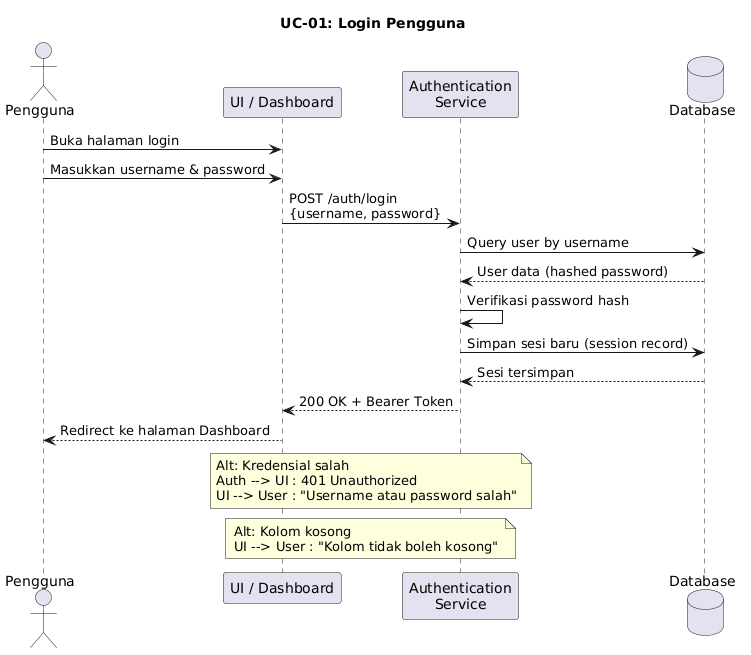
\includegraphics[width=0.85\textwidth]{images/Sequence_Diagram/sd1.png}
\end{figure}

\begin{table}[h]
  \centering
  \caption{Skenario utama dan alternatif UC-01: Login Pengguna}
  \begin{tabularx}{\textwidth}{ | X | X | }
    \hline
    \textbf{Aktor} & \textbf{Sistem} \\
    \hline
    \multicolumn{2}{|l|}{\textbf{Skenario Utama}} \\
    \hline
    1. Pengguna membuka halaman login sistem WMC. & \\
    \hline
    2. Pengguna memasukkan \textit{username} dan \textit{password}. & \\
    \hline
    & 3. Sistem memvalidasi kredensial pengguna ke basis data. \\
    \hline
    & 4. Sistem membuat sesi baru dan mengarahkan pengguna ke halaman \textit{dashboard}. \\
    \hline
    \multicolumn{2}{|l|}{\textbf{Skenario Alternatif}} \\
    \hline
    1a. Pengguna memasukkan kredensial yang salah. & \\
    \hline
    & 2a. Sistem menampilkan pesan kesalahan \enquote{Username atau password salah}. \\
    \hline
    3a. Pengguna mengosongkan salah satu atau kedua kolom. & \\
    \hline
    & 4a. Sistem menampilkan pesan validasi bahwa kolom tidak boleh kosong. \\
    \hline
  \end{tabularx}
\end{table}

\subsection{UC-02: Logout Pengguna}
Tabel \ref{tab:uc02} menyajikan skenario UC-02: Logout Pengguna.

\begin{table}[h]
  \centering
  \caption{Skenario UC-02: Logout Pengguna}
  \label{tab:uc02}
  \begin{tabularx}{\textwidth}{ | l | X | }
    \hline
    \textbf{Elemen} & \textbf{Keterangan} \\
    \hline
    ID Use Case & UC-02 \\
    \hline
    Aktor Utama & Pengguna (Operator Gudang) \\
    \hline
    Referensi SR & KF-02 \\
    \hline
    Kondisi Awal & Pengguna sudah terautentikasi dan berada di dalam sistem. \\
    \hline
    Kondisi Akhir & Sesi pengguna dihapus dan pengguna diarahkan kembali ke halaman login. \\
    \hline
    Deskripsi & Pengguna mengakhiri sesi aktif dan keluar dari sistem WMC secara aman. \\
    \hline
  \end{tabularx}
\end{table}

\begin{figure}[H]
  \caption{Diagram \textit{sequence} UC-02: Logout Pengguna}
  \label{fig:sd-uc02}
  \centering
  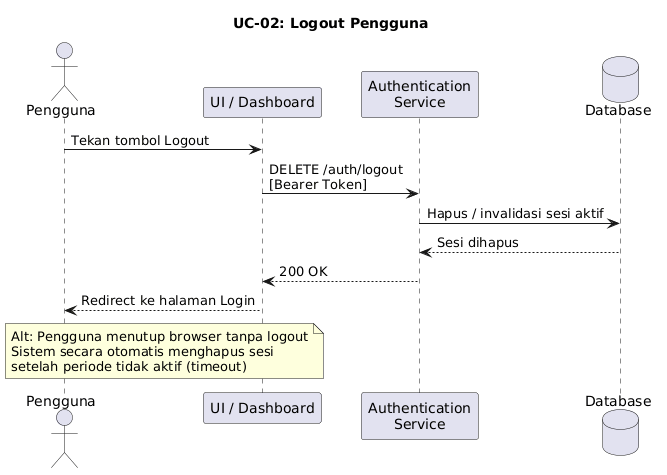
\includegraphics[width=0.85\textwidth]{images/Sequence_Diagram/sd2.png}
\end{figure}

\begin{table}[h]
  \centering
  \caption{Skenario utama dan alternatif UC-02: Logout Pengguna}
  \begin{tabularx}{\textwidth}{ | X | X | }
    \hline
    \textbf{Aktor} & \textbf{Sistem} \\
    \hline
    \multicolumn{2}{|l|}{\textbf{Skenario Utama}} \\
    \hline
    1. Pengguna menekan tombol \textit{logout} pada antarmuka sistem. & \\
    \hline
    & 2. Sistem menghapus sesi aktif pengguna dari basis data. \\
    \hline
    & 3. Sistem mengarahkan pengguna ke halaman login. \\
    \hline
    \multicolumn{2}{|l|}{\textbf{Skenario Alternatif}} \\
    \hline
    1a. Pengguna menutup \textit{browser} tanpa menekan \textit{logout}. & \\
    \hline
    & 2a. Sistem secara otomatis menghapus sesi setelah periode tidak aktif. \\
    \hline
  \end{tabularx}
\end{table}

\subsection{UC-03: Daftar Barang}
Tabel \ref{tab:uc03} menyajikan skenario UC-03: Daftar Barang.

\begin{table}[h]
  \centering
  \caption{Skenario UC-03: Daftar Barang}
  \label{tab:uc03}
  \begin{tabularx}{\textwidth}{ | l | X | }
    \hline
    \textbf{Elemen} & \textbf{Keterangan} \\
    \hline
    ID Use Case & UC-03 \\
    \hline
    Aktor Utama & Pengguna (Operator Gudang) \\
    \hline
    Referensi SR & KF-03 \\
    \hline
    Kondisi Awal & Pengguna sudah terautentikasi dan berada di halaman inventori. \\
    \hline
    Kondisi Akhir & Daftar barang ditampilkan beserta informasi ringkas setiap barang. \\
    \hline
    Deskripsi & Pengguna mengakses halaman inventori untuk melihat seluruh barang yang tersedia di gudang beserta informasi ringkasnya. \\
    \hline
  \end{tabularx}
\end{table}

\begin{figure}[H]
  \caption{Diagram \textit{sequence} UC-03: Daftar Barang}
  \label{fig:sd-uc03}
  \centering
  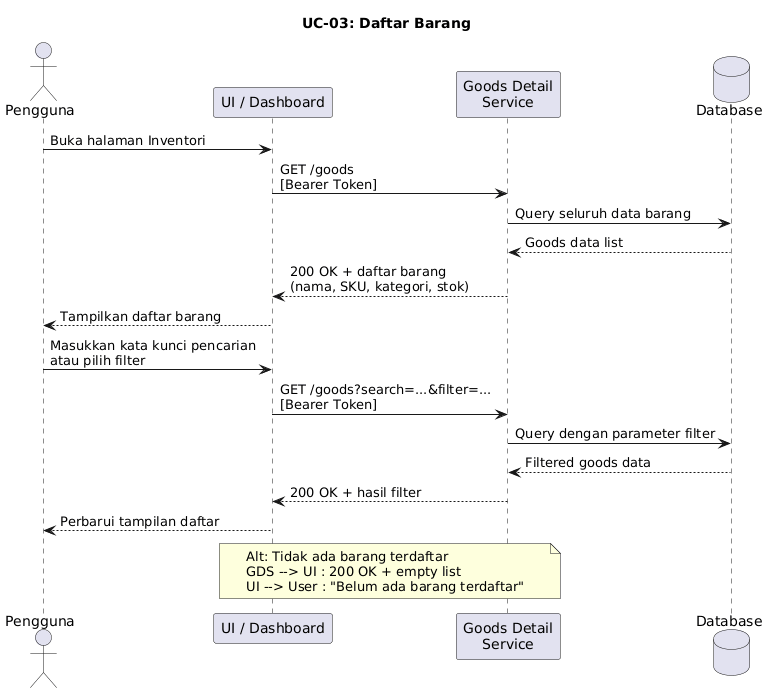
\includegraphics[width=0.85\textwidth]{images/Sequence_Diagram/sd3.png}
\end{figure}

\begin{table}[h]
  \centering
  \caption{Skenario utama dan alternatif UC-03: Daftar Barang}
  \begin{tabularx}{\textwidth}{ | X | X | }
    \hline
    \textbf{Aktor} & \textbf{Sistem} \\
    \hline
    \multicolumn{2}{|l|}{\textbf{Skenario Utama}} \\
    \hline
    1. Pengguna membuka halaman daftar inventori barang. & \\
    \hline
    & 2. Sistem mengambil data seluruh barang dari basis data. \\
    \hline
    & 3. Sistem menampilkan daftar barang dengan informasi: nama, SKU, kategori, dan stok. \\
    \hline
    4. Pengguna dapat menggunakan fitur pencarian atau \textit{filter} untuk menyempurnakan tampilan daftar. & \\
    \hline
    & 5. Sistem memperbarui tampilan daftar sesuai kriteria pencarian atau \textit{filter}. \\
    \hline
    \multicolumn{2}{|l|}{\textbf{Skenario Alternatif}} \\
    \hline
    1a. Tidak ada barang yang terdaftar di sistem. & \\
    \hline
    & 2a. Sistem menampilkan pesan \enquote{Belum ada barang terdaftar}. \\
    \hline
  \end{tabularx}
\end{table}

\subsection{UC-04: Detail Informasi Barang}
Tabel \ref{tab:uc04} menyajikan skenario UC-04: Detail Informasi Barang.

\begin{table}[h]
  \centering
  \caption{Skenario UC-04: Detail Informasi Barang}
  \label{tab:uc04}
  \begin{tabularx}{\textwidth}{ | l | X | }
    \hline
    \textbf{Elemen} & \textbf{Keterangan} \\
    \hline
    ID Use Case & UC-04 \\
    \hline
    Aktor Utama & Pengguna (Operator Gudang) \\
    \hline
    Referensi SR & KF-04 \\
    \hline
    Kondisi Awal & Pengguna berada di halaman daftar inventori barang. \\
    \hline
    Kondisi Akhir & Detail lengkap barang ditampilkan kepada pengguna. \\
    \hline
    Deskripsi & Pengguna memilih salah satu barang untuk melihat informasi lengkap, termasuk atribut, dimensi, dan riwayat pergerakan barang tersebut. \\
    \hline
  \end{tabularx}
\end{table}

\begin{figure}[H]
  \caption{Diagram \textit{sequence} UC-04: Detail Informasi Barang}
  \label{fig:sd-uc04}
  \centering
  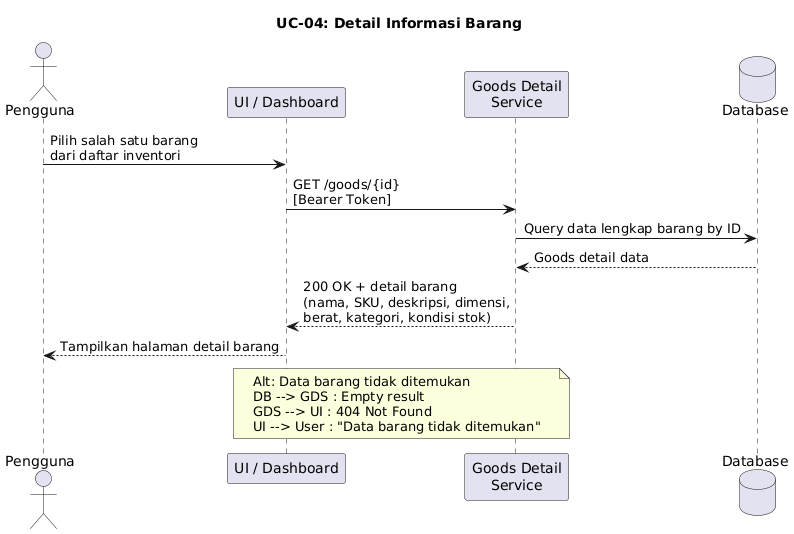
\includegraphics[width=0.85\textwidth]{images/Sequence_Diagram/sd4.png}
\end{figure}

\begin{table}[h]
  \centering
  \caption{Skenario utama dan alternatif UC-04: Detail Informasi Barang}
  \begin{tabularx}{\textwidth}{ | X | X | }
    \hline
    \textbf{Aktor} & \textbf{Sistem} \\
    \hline
    \multicolumn{2}{|l|}{\textbf{Skenario Utama}} \\
    \hline
    1. Pengguna memilih salah satu barang dari daftar inventori. & \\
    \hline
    & 2. Sistem mengambil data lengkap barang dari basis data berdasarkan ID barang. \\
    \hline
    & 3. Sistem menampilkan halaman detail barang berisi: nama, SKU, deskripsi, dimensi, berat, kategori, dan stok saat ini. \\
    \hline
    \multicolumn{2}{|l|}{\textbf{Skenario Alternatif}} \\
    \hline
    1a. Data barang tidak ditemukan (misal: barang telah dihapus). & \\
    \hline
    & 2a. Sistem menampilkan pesan \enquote{Data barang tidak ditemukan}. \\
    \hline
  \end{tabularx}
\end{table}

\subsection{UC-05: Lokasi Fisik Barang}
Tabel \ref{tab:uc05} menyajikan skenario UC-05: Lokasi Fisik Barang.

\begin{table}[h]
  \centering
  \caption{Skenario UC-05: Lokasi Fisik Barang}
  \label{tab:uc05}
  \begin{tabularx}{\textwidth}{ | l | X | }
    \hline
    \textbf{Elemen} & \textbf{Keterangan} \\
    \hline
    ID Use Case & UC-05 \\
    \hline
    Aktor Utama & Pengguna (Operator Gudang) \\
    \hline
    Referensi SR & KF-05 \\
    \hline
    Kondisi Awal & Pengguna berada di halaman detail suatu barang. \\
    \hline
    Kondisi Akhir & Lokasi penyimpanan fisik barang di gudang ditampilkan kepada pengguna. \\
    \hline
    Deskripsi & Pengguna melihat informasi lokasi penyimpanan fisik suatu barang di dalam gudang, termasuk zona, rak, dan slot penyimpanan. \\
    \hline
  \end{tabularx}
\end{table}

\begin{figure}[H]
  \caption{Diagram \textit{sequence} UC-05: Lokasi Fisik Barang}
  \label{fig:sd-uc05}
  \centering
  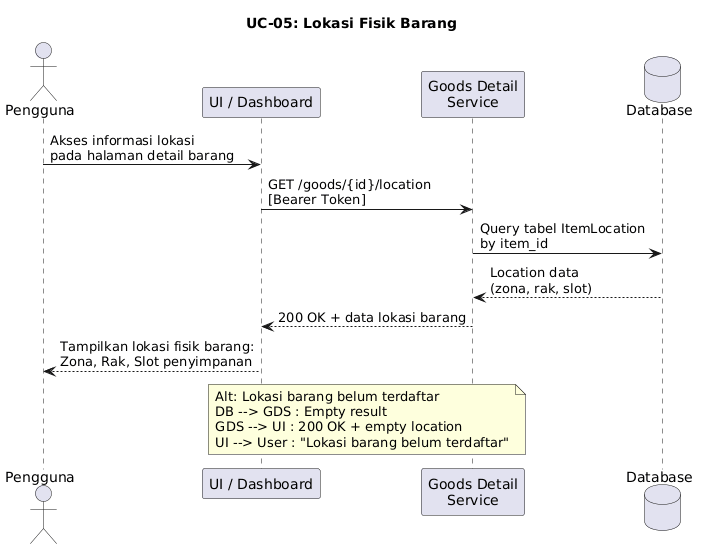
\includegraphics[width=0.85\textwidth]{images/Sequence_Diagram/sd5.png}
\end{figure}

\begin{table}[h]
  \centering
  \caption{Skenario utama dan alternatif UC-05: Lokasi Fisik Barang}
  \begin{tabularx}{\textwidth}{ | X | X | }
    \hline
    \textbf{Aktor} & \textbf{Sistem} \\
    \hline
    \multicolumn{2}{|l|}{\textbf{Skenario Utama}} \\
    \hline
    1. Pengguna mengakses informasi lokasi pada halaman detail barang. & \\
    \hline
    & 2. Sistem mengambil data lokasi barang dari tabel \textit{ItemLocation} berdasarkan ID barang. \\
    \hline
    & 3. Sistem menampilkan informasi lokasi: zona, rak (\textit{rack}), dan slot penyimpanan. \\
    \hline
    \multicolumn{2}{|l|}{\textbf{Skenario Alternatif}} \\
    \hline
    1a. Barang tidak memiliki lokasi yang terdaftar. & \\
    \hline
    & 2a. Sistem menampilkan pesan \enquote{Lokasi barang belum terdaftar}. \\
    \hline
  \end{tabularx}
\end{table}

\subsection{UC-06: Pembuatan Order Picking}
Tabel \ref{tab:uc06} menyajikan skenario UC-06: Pembuatan Order Picking.

\begin{table}[h]
  \centering
  \caption{Skenario UC-06: Pembuatan Order Picking}
  \label{tab:uc06}
  \begin{tabularx}{\textwidth}{ | l | X | }
    \hline
    \textbf{Elemen} & \textbf{Keterangan} \\
    \hline
    ID Use Case & UC-06 \\
    \hline
    Aktor Utama & Pengguna (Operator Gudang) \\
    \hline
    Referensi SR & KF-06 \\
    \hline
    Kondisi Awal & Pengguna sudah terautentikasi dan berada di halaman pembuatan \textit{order}. \\
    \hline
    Kondisi Akhir & \textit{Order picking} berhasil dibuat dan sistem menugaskan robot untuk memproses \textit{order}. \\
    \hline
    Deskripsi & Pengguna membuat \textit{order picking} untuk meminta robot mengambil barang dari lokasi penyimpanan ke titik keluaran gudang. \\
    \hline
  \end{tabularx}
\end{table}

\begin{figure}[H]
  \caption{Diagram \textit{sequence} UC-06: Pembuatan Order Picking}
  \label{fig:sd-uc06}
  \centering
  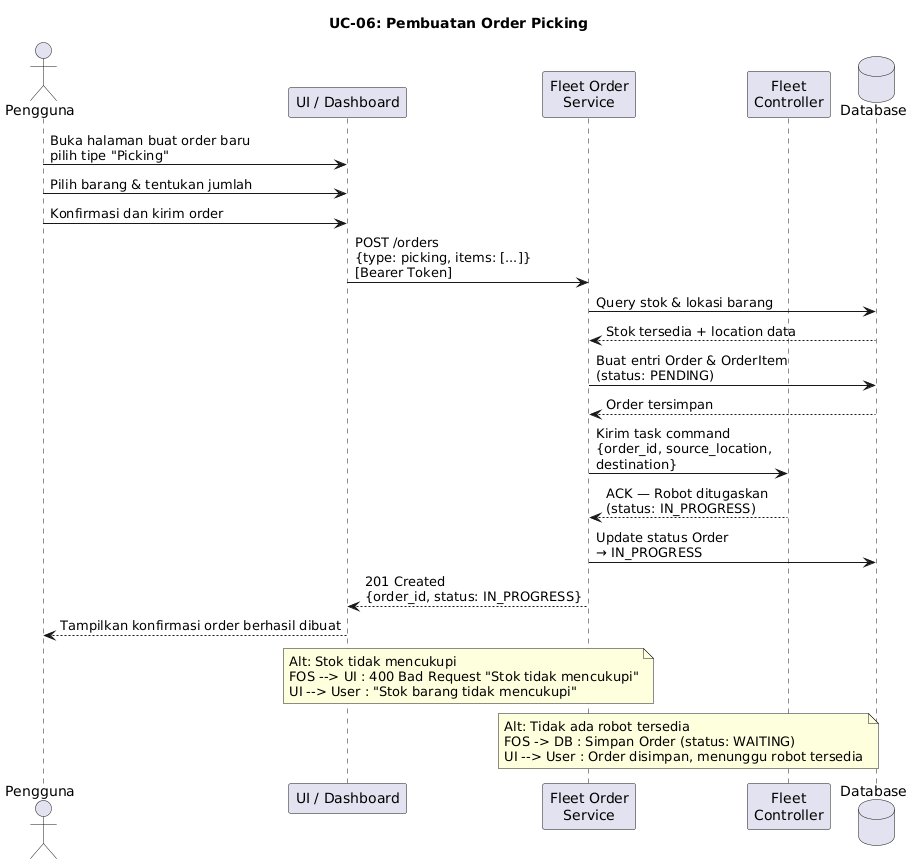
\includegraphics[width=0.85\textwidth]{images/Sequence_Diagram/sd6.png}
\end{figure}

\begin{table}[h]
  \centering
  \caption{Skenario utama dan alternatif UC-06: Pembuatan Order Picking}
  \begin{tabularx}{\textwidth}{ | X | X | }
    \hline
    \textbf{Aktor} & \textbf{Sistem} \\
    \hline
    \multicolumn{2}{|l|}{\textbf{Skenario Utama}} \\
    \hline
    1. Pengguna membuka halaman pembuatan \textit{order} baru dan memilih tipe \enquote{Picking}. & \\
    \hline
    2. Pengguna memilih barang yang akan diambil beserta jumlahnya. & \\
    \hline
    3. Pengguna mengonfirmasi dan mengirimkan \textit{order}. & \\
    \hline
    & 4. Sistem memvalidasi ketersediaan stok barang. \\
    \hline
    & 5. Sistem membuat entri \textit{Order} dan \textit{OrderItem} di basis data dengan status \enquote{Pending}. \\
    \hline
    & 6. Sistem membuat \textit{Task} untuk robot dan menugaskan robot yang tersedia. \\
    \hline
    & 7. Sistem menampilkan konfirmasi bahwa \textit{order} berhasil dibuat. \\
    \hline
    \multicolumn{2}{|l|}{\textbf{Skenario Alternatif}} \\
    \hline
    1a. Stok barang tidak mencukupi jumlah yang diminta. & \\
    \hline
    & 2a. Sistem menampilkan pesan \enquote{Stok tidak mencukupi} dan membatalkan pembuatan \textit{order}. \\
    \hline
    3a. Tidak ada robot yang tersedia saat \textit{order} dibuat. & \\
    \hline
    & 4a. Sistem menyimpan \textit{order} dengan status \enquote{Waiting} hingga robot tersedia. \\
    \hline
  \end{tabularx}
\end{table}

\subsection{UC-07: Pembuatan Order Storing}
Tabel \ref{tab:uc07} menyajikan skenario UC-07: Pembuatan Order Storing.

\begin{table}[h]
  \centering
  \caption{Skenario UC-07: Pembuatan Order Storing}
  \label{tab:uc07}
  \begin{tabularx}{\textwidth}{ | l | X | }
    \hline
    \textbf{Elemen} & \textbf{Keterangan} \\
    \hline
    ID Use Case & UC-07 \\
    \hline
    Aktor Utama & Pengguna (Operator Gudang) \\
    \hline
    Referensi SR & KF-07 \\
    \hline
    Kondisi Awal & Pengguna sudah terautentikasi dan berada di halaman pembuatan \textit{order}. \\
    \hline
    Kondisi Akhir & \textit{Order storing} berhasil dibuat dan sistem menugaskan robot untuk memproses \textit{order}. \\
    \hline
    Deskripsi & Pengguna membuat \textit{order storing} untuk meminta robot menyimpan barang dari titik masuk ke lokasi penyimpanan yang sesuai di gudang. \\
    \hline
  \end{tabularx}
\end{table}

\begin{figure}[H]
  \caption{Diagram \textit{sequence} UC-07: Pembuatan Order Storing}
  \label{fig:sd-uc07}
  \centering
  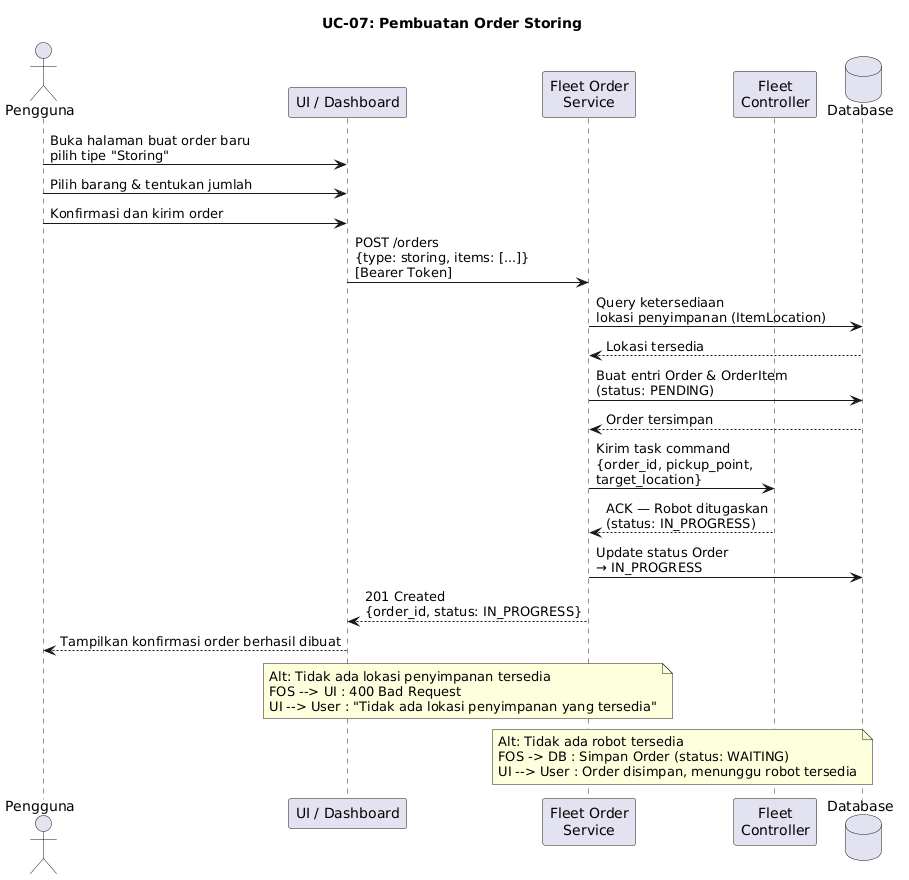
\includegraphics[width=0.85\textwidth]{images/Sequence_Diagram/sd7.png}
\end{figure}

\begin{table}[h]
  \centering
  \caption{Skenario utama dan alternatif UC-07: Pembuatan Order Storing}
  \begin{tabularx}{\textwidth}{ | X | X | }
    \hline
    \textbf{Aktor} & \textbf{Sistem} \\
    \hline
    \multicolumn{2}{|l|}{\textbf{Skenario Utama}} \\
    \hline
    1. Pengguna membuka halaman pembuatan \textit{order} baru dan memilih tipe \enquote{Storing}. & \\
    \hline
    2. Pengguna memilih barang yang akan disimpan beserta jumlahnya. & \\
    \hline
    3. Pengguna mengonfirmasi dan mengirimkan \textit{order}. & \\
    \hline
    & 4. Sistem memvalidasi bahwa lokasi penyimpanan tersedia untuk barang tersebut. \\
    \hline
    & 5. Sistem membuat entri \textit{Order} dan \textit{OrderItem} di basis data dengan status \enquote{Pending}. \\
    \hline
    & 6. Sistem membuat \textit{Task} untuk robot dan menugaskan robot yang tersedia. \\
    \hline
    & 7. Sistem menampilkan konfirmasi bahwa \textit{order} berhasil dibuat. \\
    \hline
    \multicolumn{2}{|l|}{\textbf{Skenario Alternatif}} \\
    \hline
    1a. Tidak ada lokasi penyimpanan yang tersedia. & \\
    \hline
    & 2a. Sistem menampilkan pesan \enquote{Tidak ada lokasi penyimpanan yang tersedia} dan membatalkan \textit{order}. \\
    \hline
    3a. Tidak ada robot yang tersedia saat \textit{order} dibuat. & \\
    \hline
    & 4a. Sistem menyimpan \textit{order} dengan status \enquote{Waiting} hingga robot tersedia. \\
    \hline
  \end{tabularx}
\end{table}

\subsection{UC-08: Daftar dan Status Order}
Tabel \ref{tab:uc08} menyajikan skenario UC-08: Daftar dan Status Order.

\begin{table}[h]
  \centering
  \caption{Skenario UC-08: Daftar dan Status Order}
  \label{tab:uc08}
  \begin{tabularx}{\textwidth}{ | l | X | }
    \hline
    \textbf{Elemen} & \textbf{Keterangan} \\
    \hline
    ID Use Case & UC-08 \\
    \hline
    Aktor Utama & Pengguna (Operator Gudang) \\
    \hline
    Referensi SR & KF-08 \\
    \hline
    Kondisi Awal & Pengguna sudah terautentikasi dan berada di halaman manajemen \textit{order}. \\
    \hline
    Kondisi Akhir & Daftar \textit{order} beserta status terkini ditampilkan kepada pengguna. \\
    \hline
    Deskripsi & Pengguna melihat seluruh daftar \textit{order} yang telah dibuat beserta status perkembangannya, termasuk \textit{order} yang sedang berjalan, selesai, maupun ditunda. \\
    \hline
  \end{tabularx}
\end{table}

\begin{figure}[H]
  \caption{Diagram \textit{sequence} UC-08: Daftar dan Status Order}
  \label{fig:sd-uc08}
  \centering
  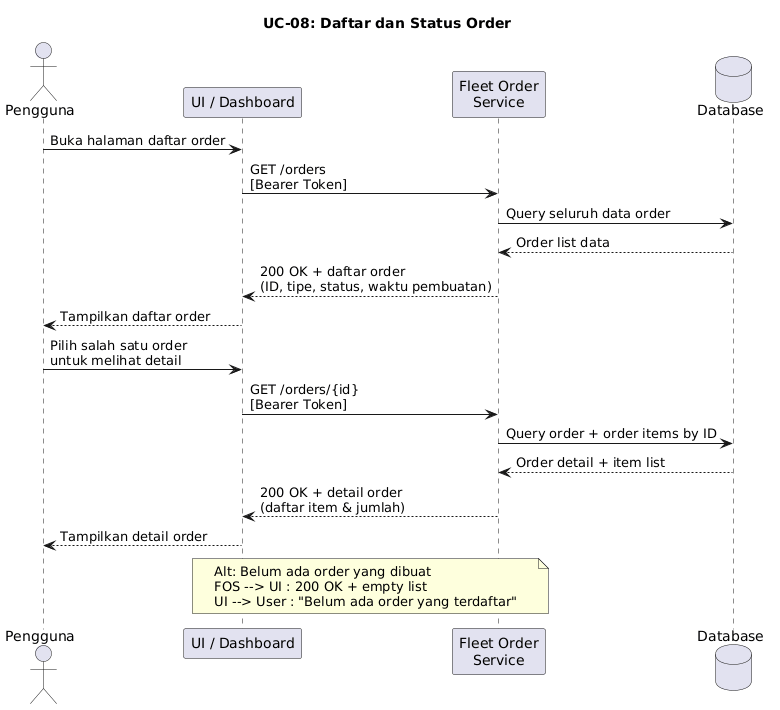
\includegraphics[width=0.85\textwidth]{images/Sequence_Diagram/sd8.png}
\end{figure}

\begin{table}[h]
  \centering
  \caption{Skenario utama dan alternatif UC-08: Daftar dan Status Order}
  \begin{tabularx}{\textwidth}{ | X | X | }
    \hline
    \textbf{Aktor} & \textbf{Sistem} \\
    \hline
    \multicolumn{2}{|l|}{\textbf{Skenario Utama}} \\
    \hline
    1. Pengguna membuka halaman daftar \textit{order}. & \\
    \hline
    & 2. Sistem mengambil data seluruh \textit{order} dari basis data. \\
    \hline
    & 3. Sistem menampilkan daftar \textit{order} dengan informasi: ID \textit{order}, tipe, status, dan waktu pembuatan. \\
    \hline
    4. Pengguna dapat memilih salah satu \textit{order} untuk melihat detail barang dalam \textit{order} tersebut. & \\
    \hline
    & 5. Sistem menampilkan detail \textit{order} berisi daftar \textit{item} dan jumlahnya. \\
    \hline
    \multicolumn{2}{|l|}{\textbf{Skenario Alternatif}} \\
    \hline
    1a. Belum ada \textit{order} yang pernah dibuat. & \\
    \hline
    & 2a. Sistem menampilkan pesan \enquote{Belum ada order yang terdaftar}. \\
    \hline
  \end{tabularx}
\end{table}

\subsection{UC-09: Pemantauan Status Task}
Tabel \ref{tab:uc09} menyajikan skenario UC-09: Pemantauan Status Task.

\begin{table}[h]
  \centering
  \caption{Skenario UC-09: Pemantauan Status Task}
  \label{tab:uc09}
  \begin{tabularx}{\textwidth}{ | l | X | }
    \hline
    \textbf{Elemen} & \textbf{Keterangan} \\
    \hline
    ID Use Case & UC-09 \\
    \hline
    Aktor Utama & Pengguna (Operator Gudang) \\
    \hline
    Referensi SR & KF-09 \\
    \hline
    Kondisi Awal & Pengguna sudah terautentikasi dan berada di halaman pemantauan operasional. \\
    \hline
    Kondisi Akhir & Status terkini seluruh \textit{task} robot ditampilkan kepada pengguna secara \textit{real-time}. \\
    \hline
    Deskripsi & Pengguna memantau status seluruh \textit{task} yang sedang dieksekusi oleh robot, termasuk informasi kemajuan dan detail \textit{task} terkait \textit{order}. \\
    \hline
  \end{tabularx}
\end{table}

\begin{figure}[H]
  \caption{Diagram \textit{sequence} UC-09: Pemantauan Status Task}
  \label{fig:sd-uc09}
  \centering
  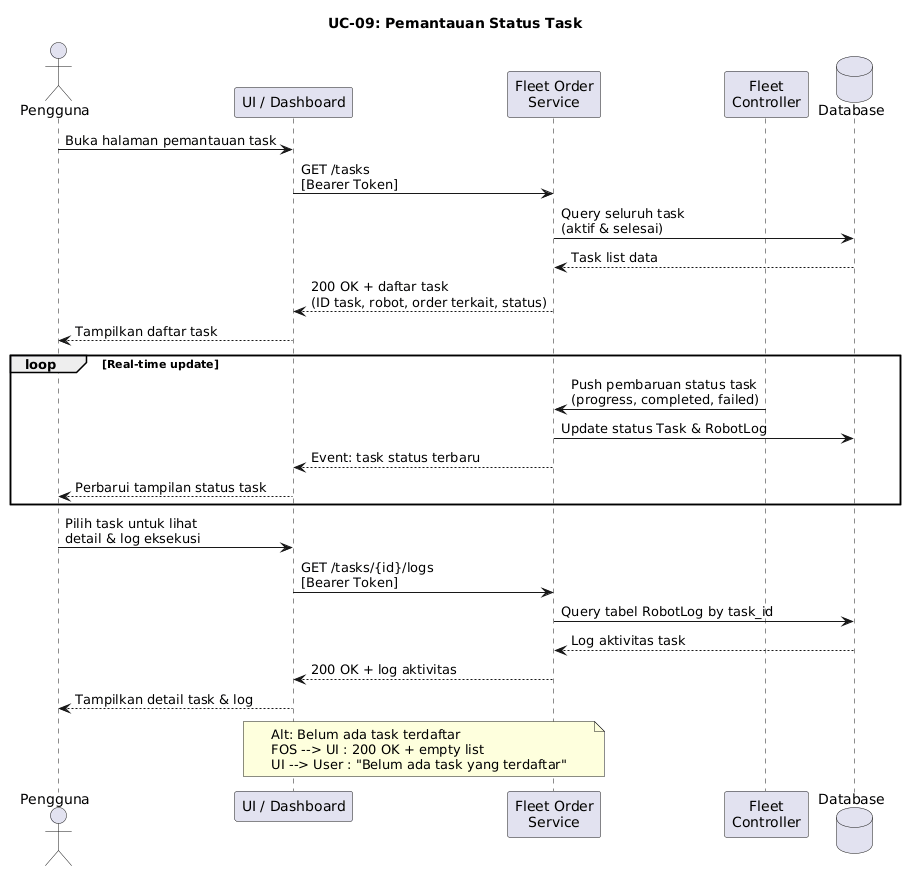
\includegraphics[width=0.85\textwidth]{images/Sequence_Diagram/sd9.png}
\end{figure}

\begin{table}[h]
  \centering
  \caption{Skenario utama dan alternatif UC-09: Pemantauan Status Task}
  \begin{tabularx}{\textwidth}{ | X | X | }
    \hline
    \textbf{Aktor} & \textbf{Sistem} \\
    \hline
    \multicolumn{2}{|l|}{\textbf{Skenario Utama}} \\
    \hline
    1. Pengguna membuka halaman pemantauan \textit{task}. & \\
    \hline
    & 2. Sistem mengambil data seluruh \textit{task} aktif dan selesai dari basis data. \\
    \hline
    & 3. Sistem menampilkan daftar \textit{task} dengan informasi: ID \textit{task}, robot yang ditugaskan, \textit{order} terkait, status, dan waktu mulai. \\
    \hline
    4. Pengguna dapat memilih \textit{task} untuk melihat detail dan log eksekusinya. & \\
    \hline
    & 5. Sistem menampilkan detail \textit{task} beserta log aktivitas dari tabel \textit{RobotLog}. \\
    \hline
    \multicolumn{2}{|l|}{\textbf{Skenario Alternatif}} \\
    \hline
    1a. Tidak ada \textit{task} yang sedang aktif maupun selesai. & \\
    \hline
    & 2a. Sistem menampilkan pesan \enquote{Belum ada task yang terdaftar}. \\
    \hline
  \end{tabularx}
\end{table}

\subsection{UC-10: Pemantauan Status Robot}
Tabel \ref{tab:uc10} menyajikan skenario UC-10: Pemantauan Status Robot.

\begin{table}[h]
  \centering
  \caption{Skenario UC-10: Pemantauan Status Robot}
  \label{tab:uc10}
  \begin{tabularx}{\textwidth}{ | l | X | }
    \hline
    \textbf{Elemen} & \textbf{Keterangan} \\
    \hline
    ID Use Case & UC-10 \\
    \hline
    Aktor Utama & Pengguna (Operator Gudang) \\
    \hline
    Referensi SR & KF-10 \\
    \hline
    Kondisi Awal & Pengguna sudah terautentikasi dan berada di halaman pemantauan operasional. \\
    \hline
    Kondisi Akhir & Status terkini seluruh robot dalam sistem ditampilkan kepada pengguna secara \textit{real-time}. \\
    \hline
    Deskripsi & Pengguna memantau kondisi dan status operasional seluruh robot yang terdaftar dalam sistem WMC, termasuk posisi, status baterai, dan aktivitas saat ini. \\
    \hline
  \end{tabularx}
\end{table}

\begin{figure}[H]
  \caption{Diagram \textit{sequence} UC-10: Pemantauan Status Robot}
  \label{fig:sd-uc10}
  \centering
  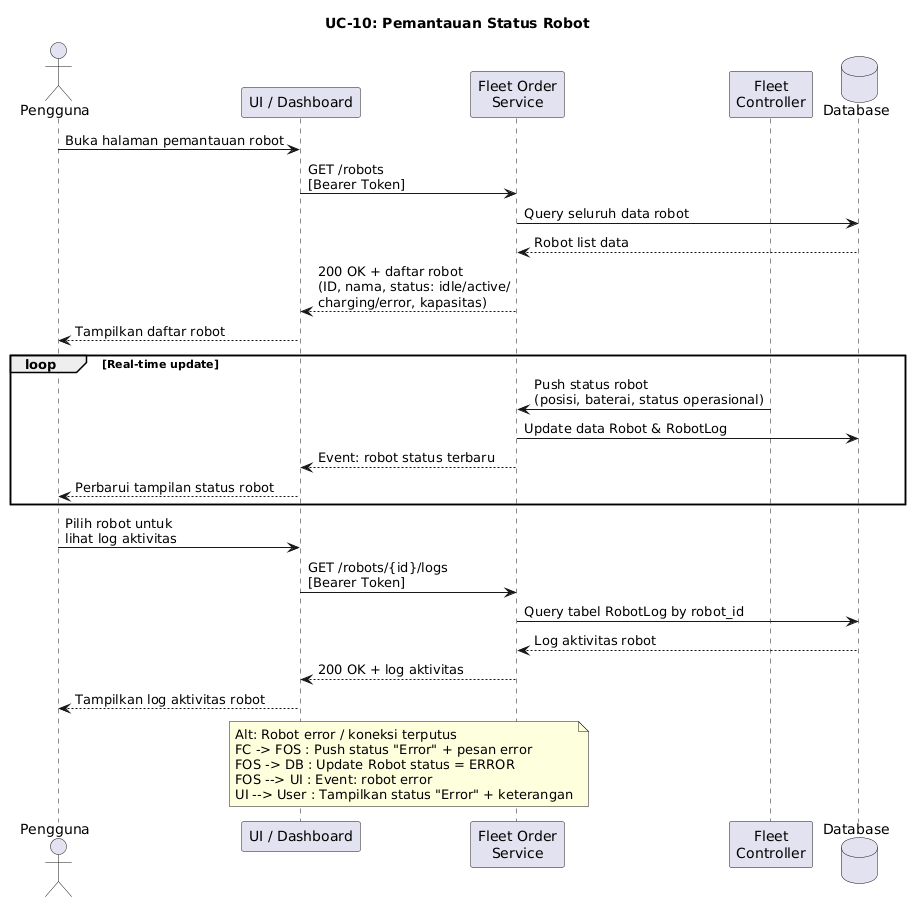
\includegraphics[width=0.85\textwidth]{images/Sequence_Diagram/sd10.png}
\end{figure}

\begin{table}[h]
  \centering
  \caption{Skenario utama dan alternatif UC-10: Pemantauan Status Robot}
  \begin{tabularx}{\textwidth}{ | X | X | }
    \hline
    \textbf{Aktor} & \textbf{Sistem} \\
    \hline
    \multicolumn{2}{|l|}{\textbf{Skenario Utama}} \\
    \hline
    1. Pengguna membuka halaman pemantauan robot. & \\
    \hline
    & 2. Sistem mengambil data seluruh robot dari basis data. \\
    \hline
    & 3. Sistem menampilkan daftar robot dengan informasi: ID robot, nama, status (\textit{idle}/\textit{active}/\textit{charging}/\textit{error}), dan \textit{task} aktif (jika ada). \\
    \hline
    4. Pengguna dapat memilih robot untuk melihat log aktivitas lengkap. & \\
    \hline
    & 5. Sistem menampilkan log aktivitas robot dari tabel \textit{RobotLog}. \\
    \hline
    \multicolumn{2}{|l|}{\textbf{Skenario Alternatif}} \\
    \hline
    1a. Robot mengalami \textit{error} atau koneksi terputus. & \\
    \hline
    & 2a. Sistem menampilkan status robot sebagai \enquote{Error} dengan keterangan pesan kesalahan terakhir dari \textit{RobotLog}. \\
    \hline
  \end{tabularx}
\end{table}
